In this adaptive strategy, the VMS-based error is calculated on the initial mesh. Based on the estimated error, a nodal size field is calculated using the following equation \cite{zhang19}

\begin{equation}
\frac{e_k}{\tilde{e}_k} = \left(\frac{h_{old}}{h_{new}}\right)^{m+N/2} 
\label{eq:diez}
\end{equation}

Here, $e_k$ is the measured local error (in the $\HOne$-seminorm) at an element $k$, $\tilde{e}_k$ is the target error for an element specified by the user, $m$ is the polynomial order of the approximation space (i.e., $m=1$ for the linear finite elements used currently) , and $N$ is the number of spatial dimensions. $h_{old}$ is current size of the element, and $h_{new}$ is the desired new mesh size.
This new mesh size at the element level is assembled at the node/vertex level to perform mesh adaptation.

\begin{figure}[H]
\centering

\begin{subfigure}[b]{0.475\textwidth}
\centering
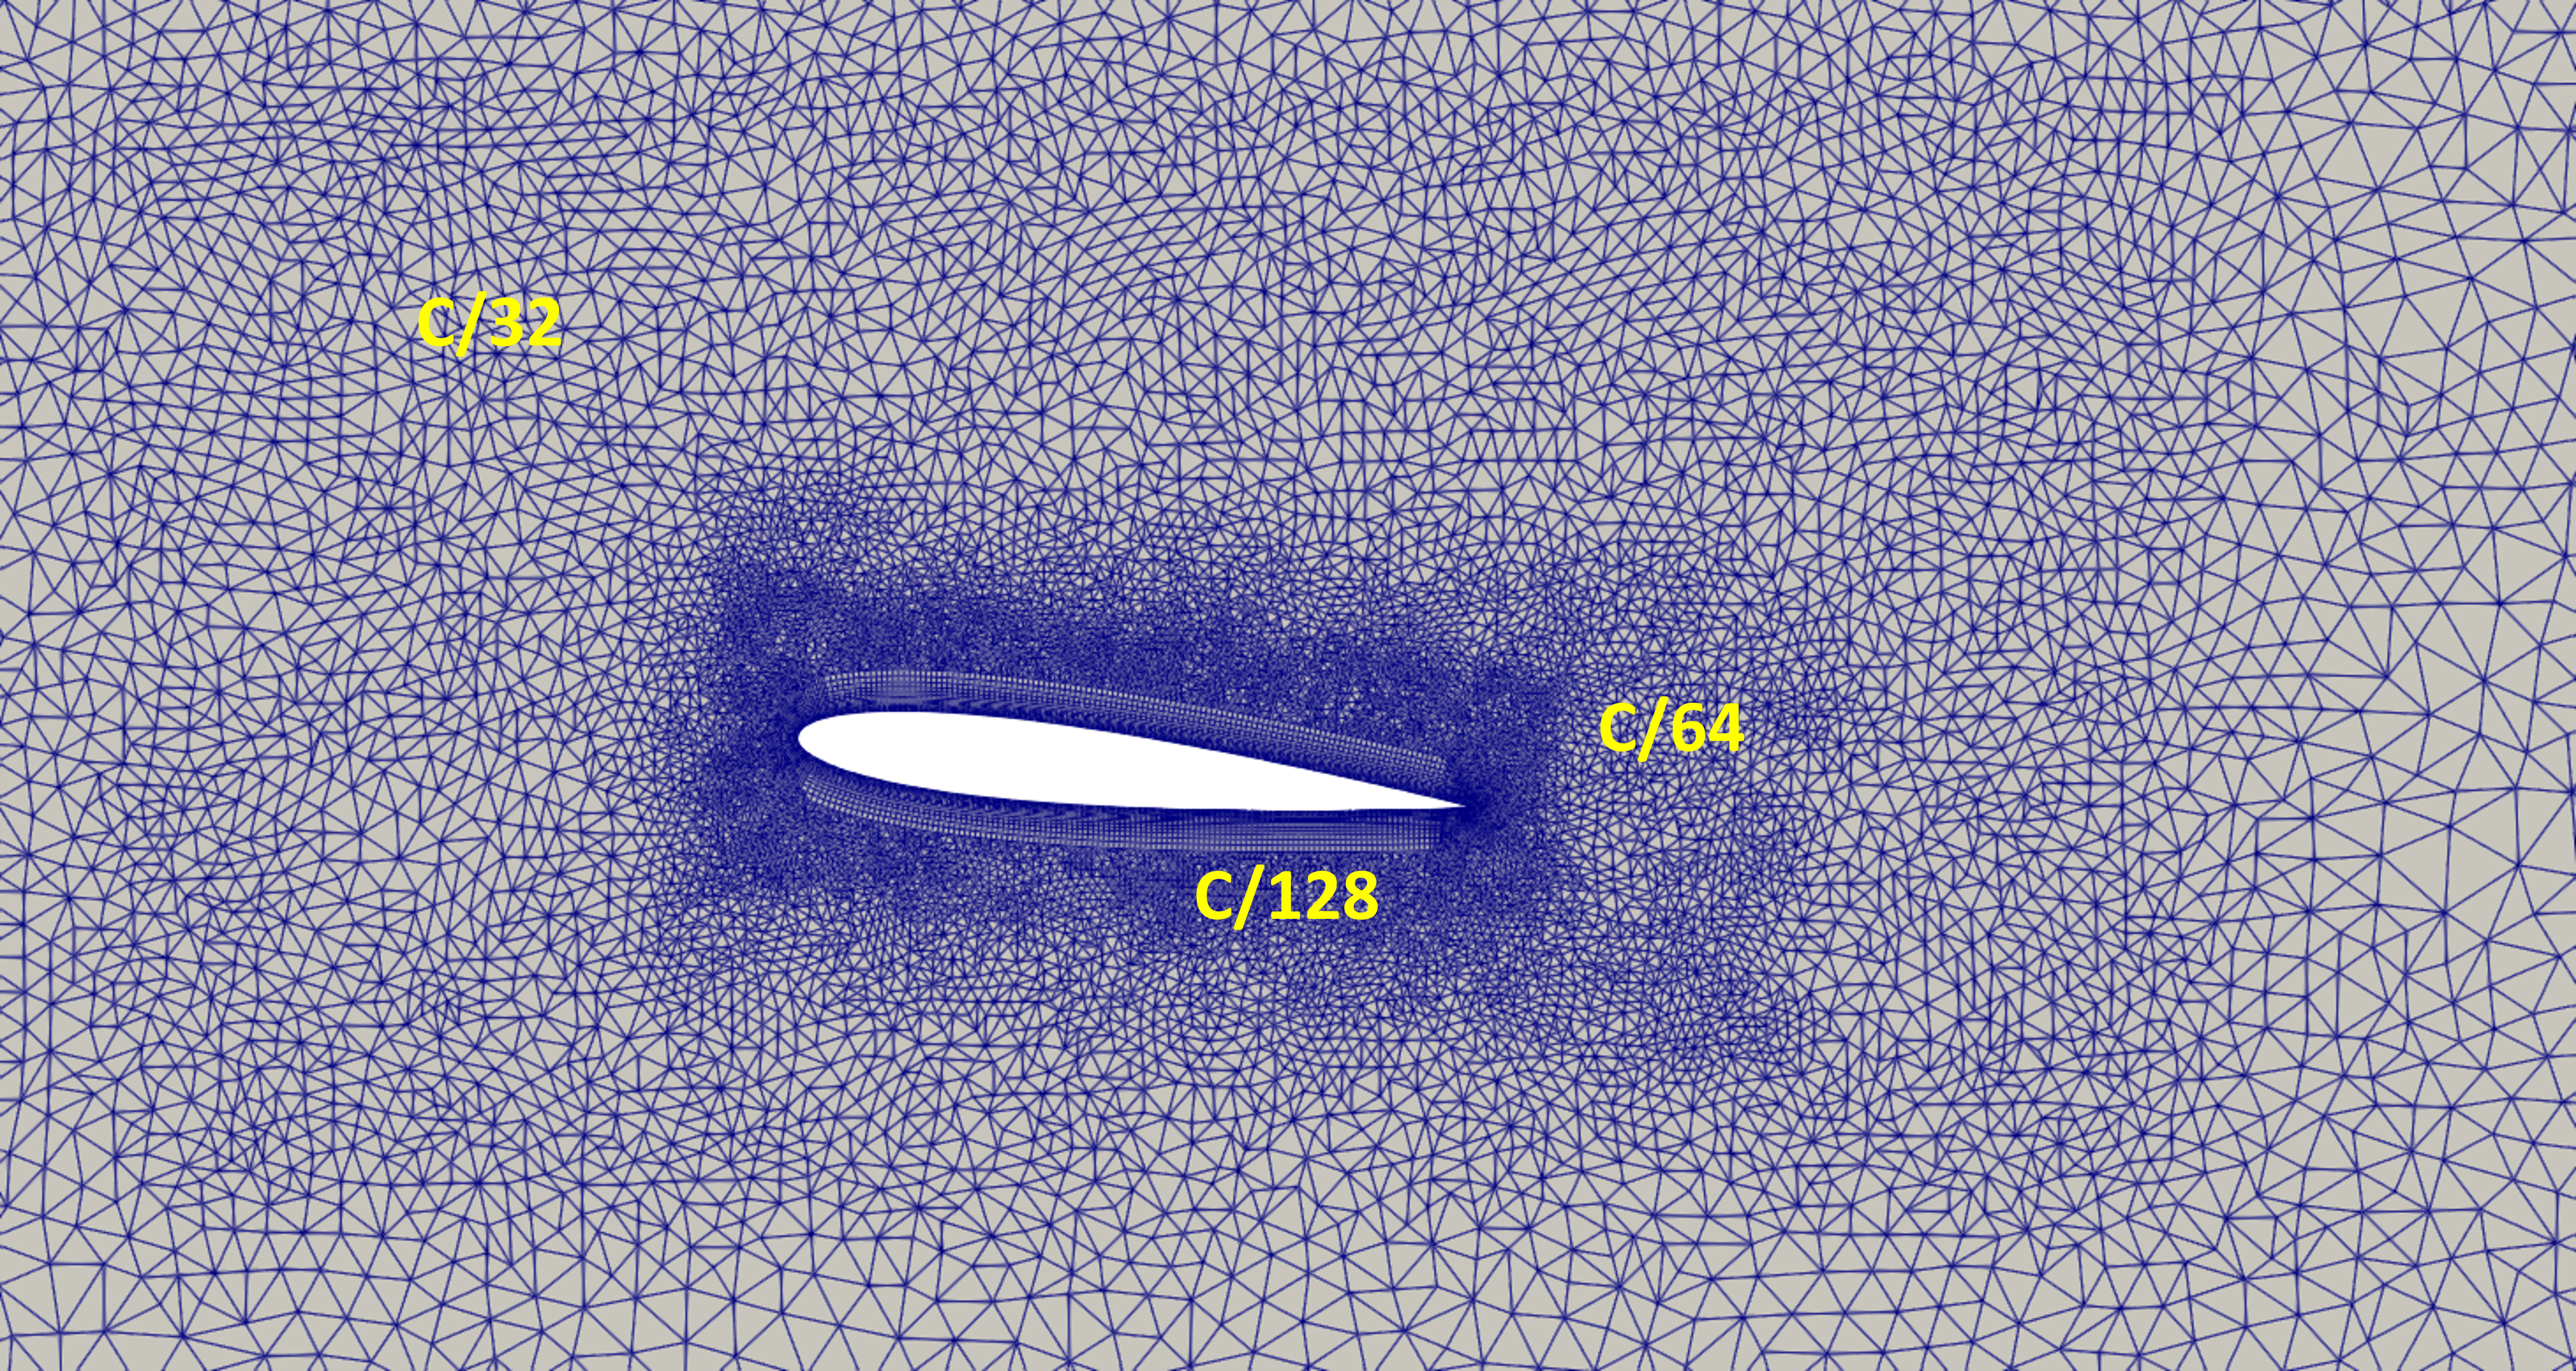
\includegraphics[width=1\textwidth]{figures/adapt_strat/Msa1_mesh.png}
\caption{Msa1\_nz50 mesh}
\label{fig:h_adapt1_mesh}
\end{subfigure}
\begin{subfigure}[b]{0.475\textwidth}
\centering
\includegraphics[width=1\textwidth]{figures/adapt_strat/Msa1_error.png}
\caption{Ms\_nz50 error field}
\label{fig:h_adapt1_error_plot}
\end{subfigure}

\caption{Mesh and estimated error for size-based refinement strategy (Msa1)}
\end{figure}

For the surging airfoil case, M0\_nz25 is used as the initial mesh (Figure \ref{fig:M0_mesh}) and the corresponding error estimated on M0\_nz25 mesh (Figure \ref{fig:M0_err_plot}) is used to calculate $h_{new}$. The mesh refinement is controlled to have a maximum refinement and maximum coarsening of a factor of 2 to avoid excessive refinement or coarsening in a local region. The mesh obtained using this strategy is shown in Figure \ref{fig:h_adapt1_mesh}. Note that in terms of mesh resolution, this mesh compares best against Mza1\_nz50 from zonal refinement strategy. This mesh consists of 2,859,450 elements, which is comparable to 2,874,300 elements for the Mza1\_n50 mesh. The major differences between the two meshes is that Mza1\_nz50 maintains the same mesh size in various zones, whereas the Ms\_a1 mesh is patchy, i.e., a uniform refinement is not maintained within regions of interest.
The corresponding estimated error for this mesh is shown in Figure \ref{fig:h_adapt1_error_plot}. Comparing the estimated error to Mza1\_nz50 mesh, higher error values are observed for Msa1\_nz50 in the LEV region, as well as in the wake of the airfoil. A more thorough comparison of results is mentioned in Section \ref{sec:results_adapt}.
